% mathbio/hw1/hw1.tex
%
% Omkar H. Ramachandran
% omkar.ramachandran@colorado.edu
%
% My solutions to HW1 of the mathbio class
%
\documentclass[english]{article}
\usepackage[T1]{fontenc}
\usepackage[latin9]{inputenc}
\usepackage{geometry}
\geometry{verbose,tmargin=1.2in,bmargin=1.2in,lmargin=1.2in,rmargin=1.2in}
\usepackage{babel}
\newcommand{\GeV}{\,{\rm GeV}}
\newcommand{\mod}{\,{\rm mod}}
\usepackage{graphicx}
\graphicspath{{./plots/}}
\usepackage{hyperref}
\usepackage{listings}
\usepackage{color}
\usepackage{titling}
\usepackage{float}
\setlength{\droptitle}{-10em}

\lstdefinestyle{custompy}{
  belowcaptionskip=1\baselineskip,
  breaklines=true,
  frame=L,
  xleftmargin=\parindent,
  language=Python,
  showstringspaces=false,
  basicstyle=\footnotesize\ttfamily,
  keywordstyle=\bfseries\color{green},
  commentstyle=\itshape\color{red},
  identifierstyle=\color{black},
  stringstyle=\color{blue},
}

\lstset{escapechar=@,style=custompy}

\begin{document}
\title{APPM 4390: Homework 1}
\author{Omkar H. Ramachandran}
\date{}
\maketitle
Phew! That was possibly the longest homework set I've ever done in my time
here in Boulder. Had a lot of fun doing it though!
\section{Four different behaviors of the Hassell model}
\begin{figure}[H]
	\centering
	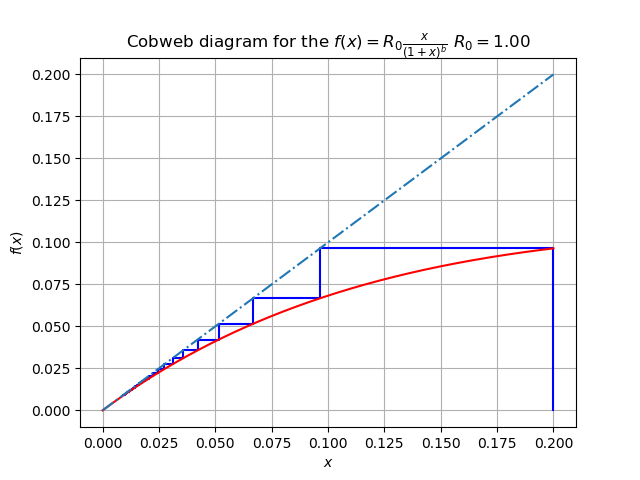
\includegraphics[width=0.45\textwidth]{plots/Problem1_R0_1.png}
	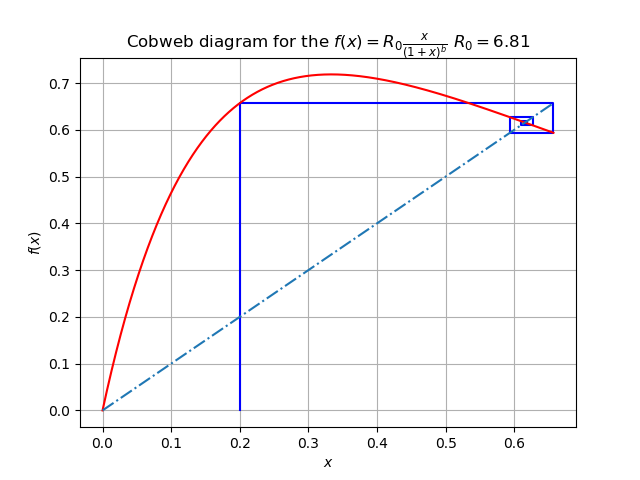
\includegraphics[width=0.45\textwidth]{plots/Problem1_R0_6p81.png}
	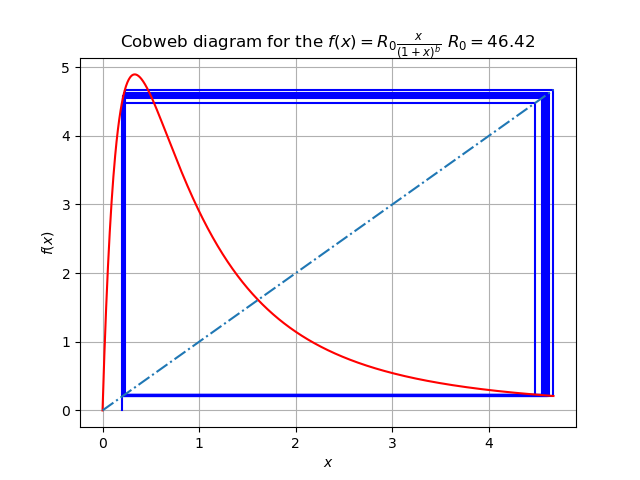
\includegraphics[width=0.45\textwidth]{plots/Problem1_R0_46p42.png}
	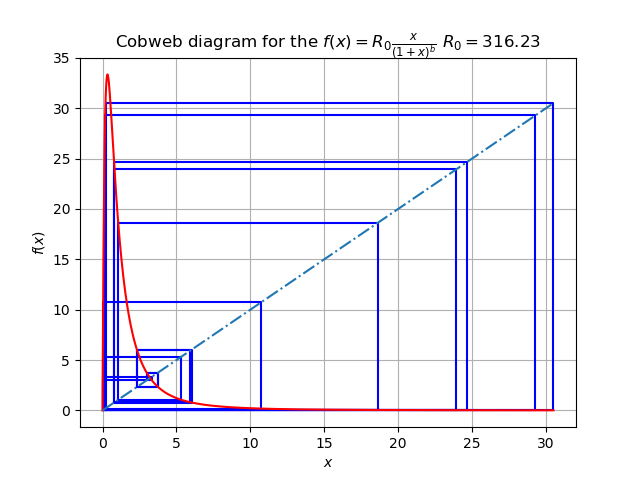
\includegraphics[width=0.45\textwidth]{plots/Problem1_R0_316p23.png}
	\caption{Cobweb plot for the Hassel model at 1. (Top Left) $R_{0} = 1$, 
	2. (Top Right) $R_{0} = 6.81$, 3. (Bottom Left) $R_{0} = 46.42$ and 4. (Bottom Right)
	$R_{0} = 316.23$}
	\label{fig:problem1}
\end{figure}


Looking at Figure \ref{fig:problem1}, it is clear that for $b=4$, choosing 
$R_{0}$ such that $\log(R_{0}) \sim \{0,1,2,3\}$ will capture the behavior of 
the system. On choosing an extremely small value for $R_{0}$ 
(Figure \ref{fig:problem1}.1), we see that $x_{n+1} < x_{n} \forall n$, thus
demonstrating monotonically stable behavior. Choosing a slightly higher value
of $R_{0}$ still keeps things stable (\ref{fig:problem1}.2), but 
$x_{n} < x_{n+2} \iff (n+1)\mod(4) \neq 0, n>0$, thus showing oscillatory
behavior that collapses -- eventually -- to a stable fixed point. Going slightly
higher, takes us to the oscillatory unstable regime (Figure \ref{fig:problem1}.3)
where we see the same oscillatory behavior as in \ref{fig:problem1}.2, but
without the function collapsing to a stable fixed point. We even see a drift
in the oscillatory path, signifying that the fixed point is unstable even in
$f^{(4)}$. Finally, in \ref{fig:problem1}.4, we see chaos, with the trajectory
following an aperiodic orbit.

\section{Britton 1.1: Nonlinear population growth}
Given the following equation:
\begin{equation}
	x_{n+1} = \frac{\lambda x_{n}}{1+x_{n}}
	\label{eq:problem2}
\end{equation}
\subsection*{a: Does this equation over or undercompensate?}
We know from Equation (1.2.4) and the explanation that immediately follows in 
EMB that the exponent in the denominator $b$ is one when the equation exactly
compensates between births and deaths.
\subsection*{b: Does it have a nontrivial steady state?}
Steady states -- or fixed points -- occur when $x_{n+1}=x_{n}$. Looking at
(\ref{eq:problem2}), we see that at a fixed point,
$$ x_{n} = \frac{x_n}{1+x_n} $$
Thus,
$$ x_n^{2} + x_{n} = \lambda x_n $$
Hence,
$$ x_n^{2} = (\lambda-1)x_n$$
Clearly, a nontrivial positive fixed point exists iff $\lambda > 1$. If this
condition is satisfied,
$$ x^{*} = \lambda - 1 $$ 
is a nontrivial steady state.

\subsection*{c and d: Discuss stability and bifurcations}
\begin{figure}[H]
	\centering
	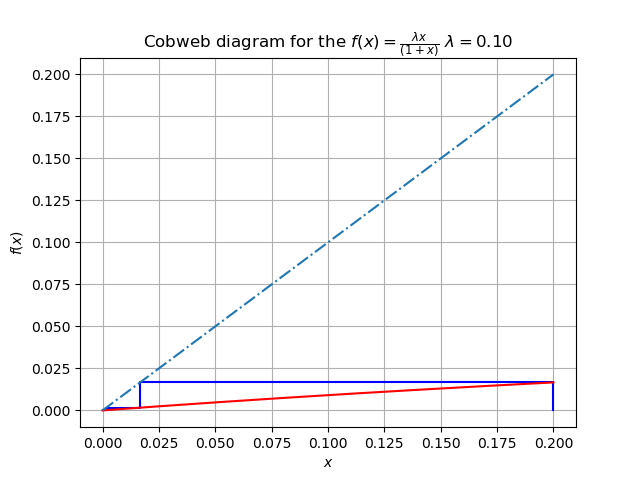
\includegraphics[width=0.45\textwidth]{plots/problem2_lambda_0p01.png}
	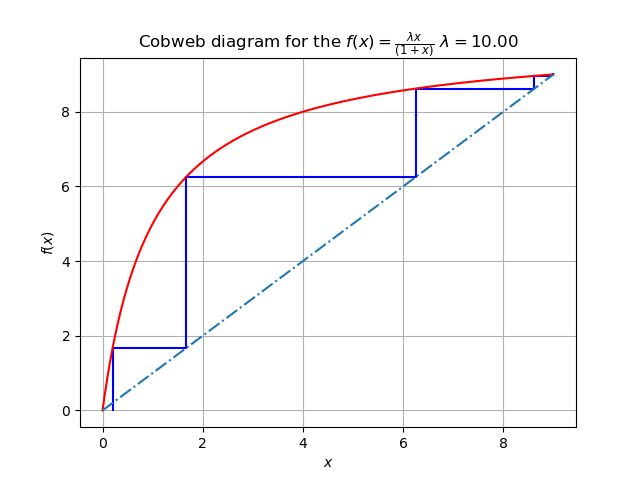
\includegraphics[width=0.45\textwidth]{plots/problem2_lambda_10.png}
	\caption{Cobweb plot of Equation \ref{eq:problem2}. 1. (Left) $\lambda = 0.01$, 
	2. (Right) $\lambda = 10$}
	\label{fig:problem2c}
\end{figure}
When $\lambda < 1$, the only fixed point is $x^{*}=0$. At this point,
$$ f'(x^{*}) = \frac{\lambda \left[(1+x^{*})-x^{*}\right]}{(1+x^{*})^{2}} $$
$$ = \frac{\lambda}{(1+x^{*})^{2}} \leq 1$$
Since $\lambda \leq 1$, this fraction as a whole has to be less than or equal
to 1. Thus, this fixed point is always stable.
When $\lambda > 1$, we have two fixed points. The derivative is obviously the
same. Thus, we have $f'(0) = \lambda > 1$, implying that 0 is an unstable fixed
point in this regime. On the other hand, $f'(\lambda-1) = 1/\lambda < 1$  which is 
always stable for $\lambda>1$. Both these behaviors are captured in Figure 
\ref{fig:problem2c}. There is a saddle-node bifurcation that occurs at $\lambda =1$.
This is evidenced by the fact that a single stable fixed point is replaced by one
stable and one unstable FP -- and the second derivative of $f$ vanishes at 
$\lambda =1$

\subsection*{e: Solve the equation exactly}
Suppose $y_n = 1/x_n$. We know that,
$$ \frac{1}{y_{n+1}} = \frac{\lambda}{1+y_n}$$
$$ \lambda y_{n+1} = y_n + 1$$
Consider a solution that looks like $y_n = Ar^{n} + B$. We now have,
$$ \lambda Ar^{n+1} = Ar^{n} + 1$$
This has to hold $\forall n$. Thus, choose two particular points $n=0$ and
$n=1$, to get
$$ \lambda Ar^{2} = Ar + 1 $$
$$ r = \frac{1}{2\lambda} \pm \sqrt{\frac{1}{4\lambda} + \frac{1}{A\lambda}}$$
Choosing only the positive root and substituting the equation for $n=0$, 
we have
$$ \sqrt{A^{2} + 4A\lambda} = A+2$$
Squaring both sides,
$$ 4A\lambda = 4A+4 $$
Thus,
$$ A = \frac{1}{\lambda-1}$$
Finally, 
$$ r = \frac{1}{2\lambda} + \sqrt{\frac{1}{4\lambda} + \frac{\lambda -1}{\lambda}}$$
If $0 < \lambda < 1$, $A < -1$, which implies that $r > 1$ (Since the term inside
the square root is large and positive). Thus $y_n \sim (>1)^{n}$, implying that
$x_n \sim 1/(>1)^{n}$ and thus decays monotonically to zero. 
On the other hand, if $\lambda \geq 1$, $r < 1$ (Both terms in $r<1$ for $\lambda \geq 1$). 
As a result, $y_n$ decreases monotonically to $1$, implying that $x_n$ increases 
with $n$. In fact, since
$$ \lim _{n\rightarrow \infty} y_n = 1 $$
ignoring $B$, we have
$$ \lim _{n\rightarrow \infty} x_n = \frac{1}{A} = \lambda -1$$
Thus, the solution monotonically increases to $\lambda -1$, agreeing with my result
in the previous section.

\section{Britton 1.4: Sterile insects}
\begin{equation}
	N_{n+1} = f(N_n) = R_0N_n\frac{N_n}{N_n+S}\frac{1}{1+aN_n}
	\label{eq:problem3}
\end{equation}
\subsection*{a: What does the $\frac{N_n}{N_n+S}$ do?}
When $N_n$ is very large,
$$ \lim _{n\rightarrow \infty}\frac{N_n}{N_n+S} = 1 $$
Demonstrating that for a huge initial insect population, sterilizing a few insects
-- in comparison -- is of no use (i.e the members we control cannot affect the
population in a meaningful way).
If, on the other hand $N_n$ is small, then
$$ \frac{N_n}{N_n+S} \sim \frac{1}{S} $$
Thus, the population we control can reduce the number of insects in the next
timestep by a factor of $S$ (i.e, we have enough sterile insects to meaningfully
control the system)
\subsection*{b: $N^{*}$ vs $S$}
\begin{figure}[H]
	\centering
	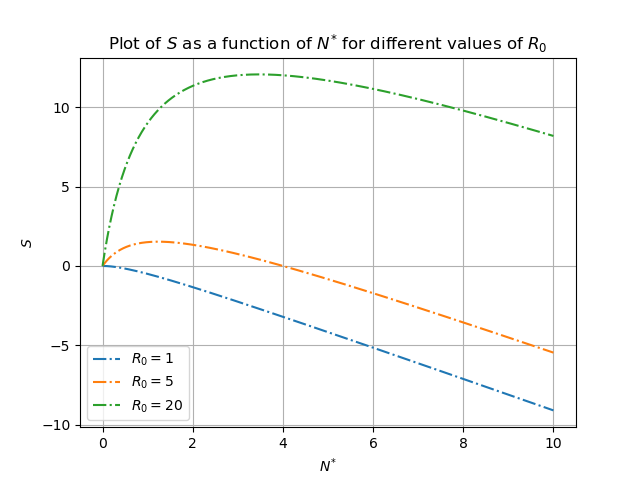
\includegraphics[width=0.45\textwidth]{plots/problem3_S_v_N.png}
	\caption{Plot of $S$ as a function of the fixed point for different growth rates}
	\label{fig:problem3_S_v_N}
\end{figure}
From equation (\ref{eq:problem3}), we see that at fixed points,
$$ 1 = R_0\frac{N^{*}}{N^{*}+S}\frac{1}{1+aN^{*}} $$
Thus,
$$ R_0N^{*} = (N^{*}+S)(1+aN^{*}) $$
Hence, denoting $N^{*}$ as $N$
$$ aN^{2}+aSN+N+S = R_0N $$
Thus,
$$S = \frac{R_0N-N-aN^{2}}{aN+1}$$
Assuming $a=1$, the plot of $S$ as a function of $N$ is shown in Figure 
\ref{fig:problem3_S_v_N}.
In essence, the larger the growth constant, the larger -- initially -- the
required $S$ to curb the population. 
However, after a while, the required $S$ drops, as the population is large
enough for competition to become significant. 
For small $R_0$, of course, no control is necessary, since the only stable
fixed point is $N=0$

\subsection*{c: Critical value of $S$}
\begin{figure}[H]
	\centering
	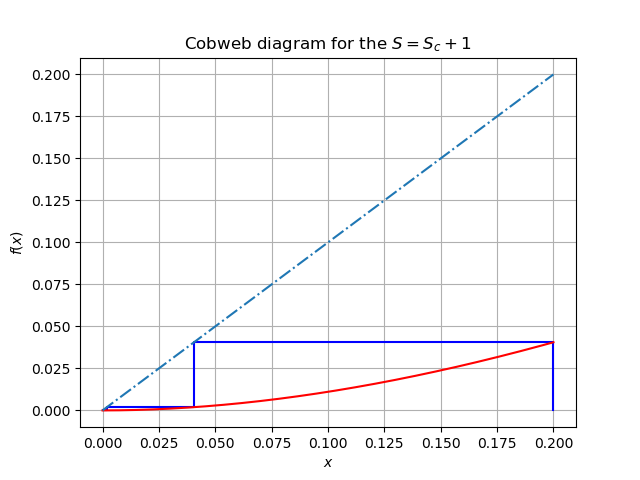
\includegraphics[width=0.45\textwidth]{plots/problem3_sgsc.png}
	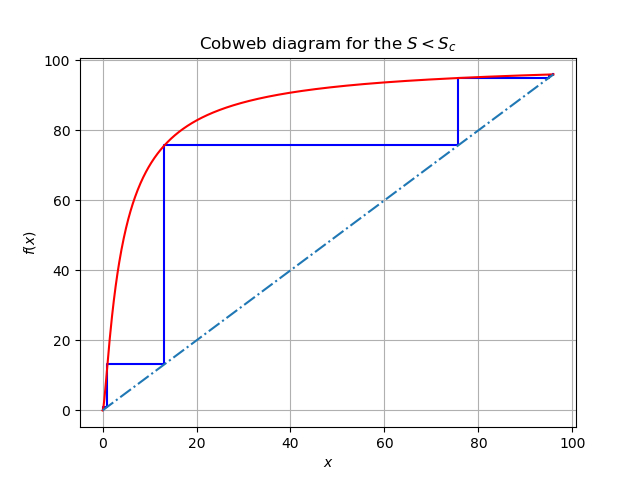
\includegraphics[width=0.45\textwidth]{plots/problem3_slsc.png}
	\caption{Cobweb plot for $S<S_c$ and $S>S_c$}
	\label{fig:problem3c_cobweb}
\end{figure}
Note: I'm assuming the question is asking for the least value of $S$ that
guarentees extinction. Given free reign of $N$, the lowest possible value
of $S$ is 0
We can find minimum values for $S$ as a function $N$ by looking for extremum
points. Thus,
$$ (aN+1)(R_0-1-2aN)-(R_0N-N-aN^{2})a = 0$$
Hence,
$$ a^{2}N^{2}-(R_0-1)+2aN=0 $$
$$ N_{max} = \frac{-2a \pm \sqrt{4a^{2}+4a^{2}(R_0-1)}}{2a^{2}}$$
Looking at the cobweb plots in Figure \ref{fig:problem3c_cobweb} that the
effect of adding $S$ is that it makes the curve dip under the line $y=x$, thus
causing the fixed point at $0$ to be stable.

\section{Britton 1.11: Fisheries}
Since the harvest rate is constant at $qEN$, the overall equation is the following:
$$ \dot{N} = rN(1-N/k)-qEN$$
\subsection*{a: Steady State equation}
Steady states occur when $\dot{N}=0$. Thus,
$$ r(1-N^{*}/k)=qE$$
Hence, we get
$$ N^{*} = k(1-qE/r)$$
\subsection*{b: Steady state yeild effort}
At steady state, the overall yeild is 
$$ Y = qEN^{*} = qEk(1-qE/r) $$
constituting the steady state yeild-effort relationship
\subsection*{c: Maximum sustainable yeild}
Maximum yeild is obtained by finding the extremum point in $Y(E)$. Thus,
$$ Y_{(E)} = qk(1-qE/r) -\frac{q^{2}Ek}{r} = 0$$
Thus,
$$ qk(1-qE_{max}/r) = \frac{q^{2}E_{max}k}{r} $$
Rearranging and crossing out terms, we have
$$ (r-qE_{max}) = qE_{max}$$
Therefore,
$$ E_{max} = \frac{r}{2q} $$
Going back to our result in the previous section, the maximum sustainable yeild
$Y_{max} = rk/4$

\section{Britton 1.14: Hutchinson's Equation}
Steady states occur when $\dot{N}=0$. Thus,
$$ (1-N(t-\tau)/k) =0 \rightarrow N(t-\tau) = k $$
and $N(t) = 0$ are steady states for the system. Taylor expanding about $k$,
we get the following:
$$ \dot{N} = -rN(t-\tau) $$
Guessing $N(t) = \exp(-\lambda \tau)$, we have
$$ \lambda = -r\exp{(-\lambda \tau)}$$
Taking the derivative of $\lambda$ wrt $\tau$, we see that
$$ \frac{d\lambda}{d\tau} = \frac{\lambda r}{\exp{(\lambda \tau)}-r\tau}$$
If the real part of $\frac{d\lambda}{d\tau}>0$ for some $\lambda = i\beta$ 
-- we can throw away the real part, since it's just a multiplicative factor
in the end --, then instabilities can form. In this case, we're interested in
$ Re(\frac{i\beta r}{\exp(i\beta\tau)-r\tau}) $. If this term is nonzero, so is it's
reciprocal. Thus,
$$ Re\left(\frac{i\beta r\exp(i\beta\tau)+i\beta r^{2}\tau}{\beta^{2}r^{2}}\right)$$
$$ = Re\left(\frac{r\sin(\beta\tau)-ir\cos(\beta\tau)+i\beta r^{2}\tau}{\beta^{2}r^{2}}\right) 
= \frac{r\sin{\beta\tau}}{\beta^{2}r^{2}} > 0$$
as long as $\beta\tau \neq n\pi$. Thus, in most cases, instabilities can form 
in the system. Looking at the fraction, as $\tau$ increases, the fraction can go
from the left of the complex plane to the right ($i\beta r^{2}\tau$), so you can
expect to see Hopf bifurcations.

\section{More delay differential equations}
The given equation is the following:
$$ \dot{x} = -ax(t)-bx(t-\tau) $$
Let us define a new function $y = x-x^{*}$. Thus,
$$ \dot{y} = -ay(t)-by(t-\tau)-C$$
\subsection*{a: Unstable equilibrium}
First, let us linearize the equation around a fixed point of $x(t)$, $x^{*}$. 
$$ \frac{dy}{dt} = \frac{\partial g(y(t),y(t+\tau))}{\partial (t+\tau)}y(t+\tau)$$
This gives us the following:
$$ \frac{dy}{dt} = -by(t-\tau)$$
Now, guess that the solution is $y(t)=\exp(\lambda t)$. Doing this yeilds the following:
$$ \lambda = -b\exp(\lambda \tau)$$
Now, guess that $\lambda = i\beta$.


\end{document}
